\documentclass{beamer}
\mode<presentation>
\usepackage{amsmath}
\usepackage{amssymb}
%\usepackage{advdate}
\usepackage{adjustbox}
\usepackage{subcaption}
\usepackage{enumitem}
\usepackage{multicol}
\usepackage{mathtools}
\usepackage{listings}
\usepackage{url}
\def\UrlBreaks{\do\/\do-}
\usetheme{metropolis}
%\usecolortheme{lily}
\setbeamertemplate{footline}
{
	\leavevmode%
	\hbox{%
		\begin{beamercolorbox}[wd=\paperwidth,ht=2.25ex,dp=1ex,right]{author in head/foot}%
			\insertframenumber{} / \inserttotalframenumber\hspace*{2ex} 
		\end{beamercolorbox}}%
		\vskip0pt%
	}
	\setbeamertemplate{navigation symbols}{}

	\providecommand{\nCr}[2]{\,^{#1}C_{#2}} % nCr
	\providecommand{\nPr}[2]{\,^{#1}P_{#2}} % nPr
	\providecommand{\mbf}{\mathbf}
	\providecommand{\pr}[1]{\ensuremath{\Pr\left(#1\right)}}
	\providecommand{\qfunc}[1]{\ensuremath{Q\left(#1\right)}}
	\providecommand{\sbrak}[1]{\ensuremath{{}\left[#1\right]}}
	\providecommand{\lsbrak}[1]{\ensuremath{{}\left[#1\right.}}
	\providecommand{\rsbrak}[1]{\ensuremath{{}\left.#1\right]}}
	\providecommand{\brak}[1]{\ensuremath{\left(#1\right)}}
	\providecommand{\lbrak}[1]{\ensuremath{\left(#1\right.}}
	\providecommand{\rbrak}[1]{\ensuremath{\left.#1\right)}}
	\providecommand{\cbrak}[1]{\ensuremath{\left\{#1\right\}}}
	\providecommand{\lcbrak}[1]{\ensuremath{\left\{#1\right.}}
	\providecommand{\rcbrak}[1]{\ensuremath{\left.#1\right\}}}
	\theoremstyle{remark}
	\newtheorem{rem}{Remark}
	\newcommand{\sgn}{\mathop{\mathrm{sgn}}}
	\providecommand{\abs}[1]{\left\vert#1\right\vert}
	\providecommand{\res}[1]{\Res\displaylimits_{#1}} 
	\providecommand{\norm}[1]{\lVert#1\rVert}
	\providecommand{\mtx}[1]{\mathbf{#1}}
	\providecommand{\mean}[1]{E\left[ #1 \right]}
	\providecommand{\fourier}{\overset{\mathcal{F}}{ \rightleftharpoons}}
	%\providecommand{\hilbert}{\overset{\mathcal{H}}{ \rightleftharpoons}}
	\providecommand{\system}{\overset{\mathcal{H}}{ \longleftrightarrow}}
	%\newcommand{\solution}[2]{\textbf{Solution:}{#1}}
	%\newcommand{\solution}{\noindent \textbf{Solution: }}
	\providecommand{\dec}[2]{\ensuremath{\overset{#1}{\underset{#2}{\gtrless}}}}
	\newcommand{\myvec}[1]{\ensuremath{\begin{pmatrix}#1\end{pmatrix}}}
		\let\vec\mathbf

		\lstset{
			%language=C,
			frame=single, 
			breaklines=true,
			columns=fullflexible
		}

		\numberwithin{equation}{section}

		\title{Sprog Presentation}
		\author{Akshara Sarma Chennubhatla,\\ EE24BTECH11003,\\IIT Hyderabad.\\}

		\date{\today} 
		\begin{document}

		\begin{frame}
			\titlepage
		\end{frame}

		\begin{frame}
			\frametitle{Problem Statement}

The sum of the perimeter of a circle and square is $k$, where $k$ is some constant. Prove that the sum of their areas is least when the side of square is double the radius of the circle.

		\end{frame}
		\subsection{Solution}
		\begin{frame}
      \frametitle{Solution}
The method used to solve this question is the gradient descent.\\
Taking the radius of the circle as $r$ and the side of the square as $a$, through given information,
\begin{align}
	2\pi r + 4a = k
\end{align}
We need to minimize
\begin{align}
	\pi r^2 + a^2
\end{align}
and prove that at the minimum sum of areas point, $a = 2r$.\\
		\end{frame}
\begin{frame}
      \frametitle{Solution}
	Substituting $\brak{0.1}$ in $\brak{0.2}$,
\begin{align}
	A\brak{r} &= \pi r^2 + \brak{\frac{k - 2\pi r}{4}}^2\\
	A\brak{r} &= \brak{\frac{\pi^2}{4} + \pi}r^2 - \frac{\pi k}{4}r + \frac{k^2}{16}
\end{align}
\end{frame}
		\begin{frame}
      \frametitle{Solution}
			Applying Gradient Descent to this function,
\begin{align}
	r_{n+1} &= r_n - \mu A^\prime\brak{r_n}\\
	A^\prime\brak{x} &= 2\brak{\frac{\pi^2}{4} + \pi}r - \frac{\pi k}{4}\\
	r_{n+1} &= r_n\brak{1 - 2\mu\brak{\frac{\pi^2}{4} + \pi}} + \frac{\mu\pi k}{4}
\end{align}
		\end{frame}
		\begin{frame}
      \frametitle{Solution}
			Applying unilateral Z-transform,
\begin{align}
	zR\brak{z} - zr_0 &= R\brak{z}\brak{1 - 2\mu\brak{\frac{\pi^2}{4} + \pi}} + \frac{\mu\pi k}{4} \frac{1}{1 - z^{-1}}\\
	R\brak{z} &= \frac{zr_0}{z - \brak{1 - 2\mu\brak{\frac{\pi^2}{4} + \pi}}} + \frac{\mu\pi k}{4} \frac{1}{1 - z^{-1}}
\end{align}
		\end{frame}
		\begin{frame}
      \frametitle{Solution}

			\begin{multline}
	R\brak{z} = \frac{zr_0}{z - \brak{1 - 2\mu\brak{\frac{\pi^2}{4} + \pi}}} + \frac{k}{10 \pi \brak{z - 1}} \\- \frac{k \brak{1 - 2\mu\brak{\frac{\pi^2}{4} + \pi}}}{10 \pi \brak{z - \brak{1 - 2\mu\brak{\frac{\pi^2}{4} + \pi}}}}\\
	R\brak{z} = \frac{r_0}{1 - z^{-1}\brak{1 - 2\mu\brak{\frac{\pi^2}{4} + \pi}}} + \frac{kz^{-1}}{10 \pi \brak{1 - z^{-1}}} \\- \frac{z^{-1}k \brak{1 - 2\mu\brak{\frac{\pi^2}{4} + \pi}}}{10 \pi \brak{1 - z^{-1}\brak{1 - 2\mu\brak{\frac{\pi^2}{4} + \pi}}}}
			\end{multline}

		\end{frame}
		\begin{frame}
      \frametitle{Solution}
			From this equation, the ROC is,
\begin{align}
	\abs{z} &> max\brak{\abs{1 - 2\mu\brak{\brak{\frac{\pi^2}{4} + \pi}}},1}\\
	\implies \abs{z} &> 1	
\end{align}
		\end{frame}
		\begin{frame}
      \frametitle{Solution}
			Assuming $\mu$ satisfies the above condition,
\begin{align}
	\lim_{n\to\infty}\norm{r_{n+1} - r_n} &= 0\\
	\lim_{n\to\infty}\norm{\frac{\mu k\pi}{4} - r_n2\mu\brak{\frac{\pi^2}{4} + \pi}} &= 0\\
	\implies \lim_{n\to\infty}\norm{r_n} &= \frac{k}{8\brak{\frac{\pi}{4} + 1}}
\end{align}
		\end{frame}
		\begin{frame}
      \frametitle{Solution}
			But, we know that,
\begin{align}
	2\pi r_n + 4a_n &= k\\
	2\pi \brak{\frac{k}{2\brak{\pi + 4}}} + 4a_n &= k\\
	\implies a_n &= \frac{k}{\pi + 4}\\
	\implies a_n &= 2r_n
\end{align}
Thus, it is proved that at minimum condition, the length of the side of the square is double the radius of the circle.
		\end{frame}
		\begin{frame}
      \frametitle{Solution}
			Below is the plot for the area vs radius graph with initial conditions as follows,
\begin{align}
	r_0 &= -10\\
	\mu &= 0.001\\
	\text{tolerance of convergence} &= 10^{-6}\\
	k &= 10\pi\\
\end{align}
The point of minima we get is,
\begin{align}
	r_{min} = 2.199416...
\end{align}
\end{frame}
\begin{frame}
      \frametitle{Plot}
	\begin{figure}[h!]
	\centering
	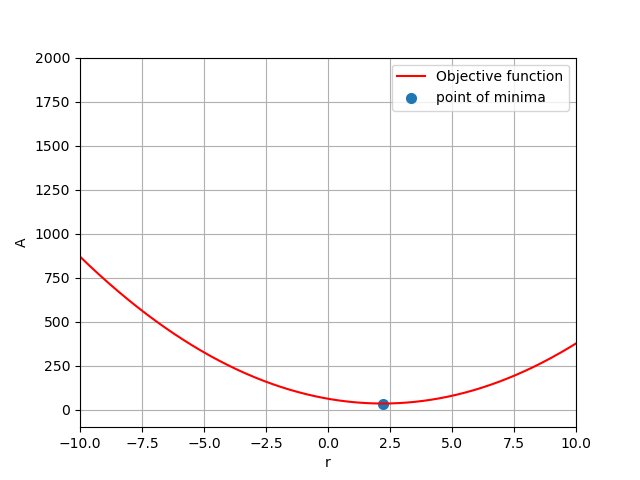
\includegraphics[width=1\columnwidth]{figs/simulated.png}
	\caption{Plot of the area vs radius}
	\label{stemplot}
\end{figure}
\end{frame}
\end{document}
